\begin{frame}[fragile]{Metrics for images}
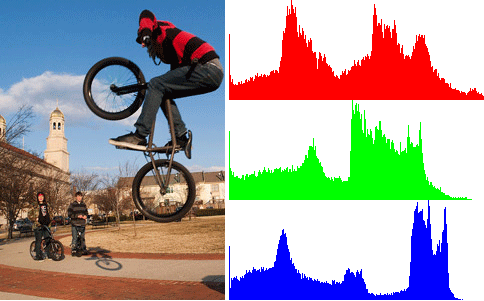
\includegraphics[width=6cm]{slides/covertree/imagehistogram2.png}
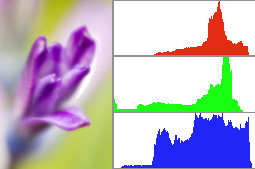
\includegraphics[width=6cm]{slides/covertree/imagehistogram3b.jpg}

\vspace{0.15in}
There are \emph{lots} of distance metrics for images.
Histogram metrics follow the two step process:
\begin{itemize}
\item generate histograms (usually of colors)
\item define a distance between histograms
\end{itemize}

Earth mover's distance is a popular but slow metric.
It runs in time $O(b^3 \log b)$, where $b$ is the size of the histogram.
(Rubner \emph{et. al.}, 1998)

\vspace{0.05in}
{\tiny
images from: \url{http://billmill.org/the_histogram.html}
}
\end{frame}


%\begin{frame}[fragile]{metrics for images}
%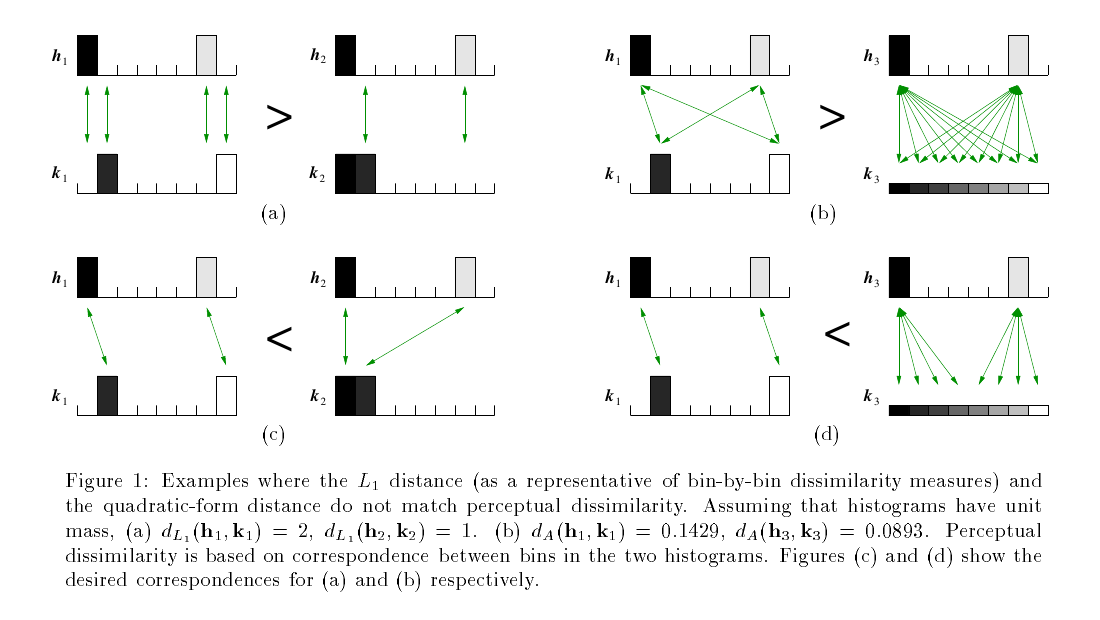
\includegraphics[width=12cm]{slides/covertree/emd.png}
%
%\end{frame}
